\section{Classification of Crystallographic Root Systems}

If $G < GL(V)$ such that $g(\Lambda) = \Lambda$ for all $g \in G$ for $\Lambda$
some lattice $\Lambda \subset V$, then $G$ is said to be crystallographic.

\begin{lemma} \label{cor19}
Let $W$ be a crystallographic finite reflection group. Then its labels must be
in $\{2, 3, 4, 6\}$.
\end{lemma}

\begin{proof}
Let $\Lambda = \sum_{i=1}^r \Z b_i$. Then the matrix $A = (a_{ij})$ of $g$ wrt
$\{b_1, \dots, b_r\}$ is an integer matrix, since $g(b_i) = \sum_{j=1}^r
a_{ij} b_j \in \Lambda$.
Hence ${\rm tr} (A) \in \Z$.
Since the trace of a linear operator is an invariant\footnote{does not depend
on the choice of basis; a change of basis corresponds to a similarity transformation
leaving the trace invariant -- ${\rm tr}(SAS^{-1}) = {\rm tr}(S){\rm tr}(A)
{\rm tr}(S^{-1}) = {\rm tr}(ASS^{-1}) = {\rm tr}(A)$}, then ${\rm tr}(g) \in \Z$.

Now choose a different basis of $V$. Let $P_{\alpha, \beta} = \Z \alpha +
\Z \beta$ for $\alpha, \beta \in \Delta, (\alpha \neq \beta)$, and
$B_{\alpha,\beta}^\perp$ a basis of $P_{\alpha, \beta}^\perp$ (the orthogonal
space to $P_{\alpha, \beta}$), and $B = \{\alpha, \beta\} \cup
B_{\alpha,\beta}^\perp$ (i.e. if $b \in B_{\alpha, \beta}^\perp$, $(b, \alpha)
= (b, \beta) = 0$).

$s_\alpha s_\beta$ acts as a rotation through $2\theta =
\frac{2\pi}{m_{\alpha \beta}}$ and fixes, pointwise $P_{\alpha, \beta}^\perp$.
With respect to our new basis $B$, $g$ has matrix representation
\[
    \begin{pmatrix}
        \cos (2\theta) & -\sin(2\theta) \\
        \sin (2\theta) & \cos(2\theta) \\
        & & 1 \\
        & & & 1 \\
        & & & & \ddots \\
        & & & & & 1
    \end{pmatrix}
\]
Hence ${\rm tr}(g) = 2 \cos 2\theta + (r-2) \in \Z$, so $2 \cos 2\theta \in \Z$,
so $m_{\alpha \beta} \in \{2,3,4,6\}$.
\end{proof}

\begin{corollary} \label{cor20}
The finite reflection groups $H_3$, $H_4$ and $I_2(m)$, unless
$m \in \{3,4,6\}$, are not crystallographic.
\end{corollary}

(Note that $I_2(3) = A_2$, $I_2(4) = B_2$. $I_2(6)$ is also called $G_2$.)
The crystallographic condition $(\alpha, \beta^\vee) \in \Z$ now makes perfect
sense.

From $(\alpha, \beta^\vee) \in \Z$, it follows that $(\alpha, \beta^\vee)
(\alpha^\vee, \beta) \in \Z$, so $4 \cos^2 \theta \in \Z$, therefore
\[ \theta \in \left\{\frac{\pi}{6}, \frac{\pi}{4}, \frac{\pi}{3}, \frac{\pi}{2},
\frac{2\pi}{3}, \frac{3\pi}{4}, \frac{5\pi}{6}\right\} \] (unless
$\alpha = \pm \beta$, in which case $\theta \in \{0, \pi\}$).

Since $\theta = \pi - \frac{\pi}{m_{\alpha \beta}}$, we have $m_{\alpha \beta}
\in \{2,3,4,6\}$. Moreover, since $s_\alpha(\beta) = \beta -
(\alpha^\vee, \beta) \alpha \in \beta + \Z \alpha$. Therefore, $\beta
= \sum_{\alpha \in \Delta} n_\alpha \alpha$, for $n_\alpha \in \Z$.
Therefore, $\Lambda = \sum_{i=1}^r \Z \alpha_i$ is fixed by $W$.

However, not just the angles are fixed, but also the relative length of the
roots: $(\alpha, \beta^\vee) = 2\frac{||\alpha||}{||\beta||} \cos \theta \in \Z$,
so adjacent roots have relative lengths $1, \sqrt{2}, \sqrt{3}$ (corresponding to
$m = 3, 4, 6$).

Revisiting our previous description of root systems, we get the following:
(note that we also annotate the vertices of the graph with the length of the
root, in red)

\begin{itemize}
\item $A_{n-1}$,
\[
\begin{picture}(5,1)(-0.3,0.1)
\put(0,0.2){\circle*{0.2}}
\put(0,0.2){\line(1,0){1}}
\put(1,0.2){\circle*{0.2}}
\put(1,0.2){\line(1,0){1}}
\put(2,0.2){\circle*{0.2}}
\put(2,0.2){\line(1,0){0.1}}
\put(2.2,0.2){\line(1,0){0.1}}
\put(2.4,0.2){\line(1,0){0.1}}
\put(2.6,0.2){\line(1,0){0.1}}
\put(2.8,0.2){\line(1,0){0.1}}
\put(3,0.2){\circle*{0.2}}
\put(3,0.2){\line(1,0){1}}
\put(4,0.2){\circle*{0.2}}
\put(-0.3,0.4){\textcolor{red}{$\sqrt{2}$}}
\put(0.7,0.4){\textcolor{red}{$\sqrt{2}$}}
\put(3.7,0.4){\textcolor{red}{$\sqrt{2}$}}
\put(-0.1,-0.3){1}
\put(3.7,-0.3){$n-1$}
\end{picture}
    \quad \quad \quad
    \Lambda = \sum_{i=1}^{n-1} \Z (\varepsilon_i - \varepsilon_{i+1}).
\]

\item $B_n$,
\[
\begin{picture}(4.3,1)(-0.3,0.1)
\put(0,0.2){\circle*{0.2}}
\put(0,0.2){\line(1,0){1}}
\put(1,0.2){\circle*{0.2}}
\put(1,0.2){\line(1,0){1}}
\put(2,0.2){\circle*{0.2}}
\put(2,0.2){\line(1,0){0.1}}
\put(2.2,0.2){\line(1,0){0.1}}
\put(2.4,0.2){\line(1,0){0.1}}
\put(2.6,0.2){\line(1,0){0.1}}
\put(2.8,0.2){\line(1,0){0.1}}
\put(3,0.2){\circle*{0.2}}
\put(3,0.2){\line(1,0){1}}
\put(4,0.2){\circle*{0.2}}
\put(-0.3,0.4){\textcolor{red}{$\sqrt{2}$}}
\put(0.7,0.4){\textcolor{red}{$\sqrt{2}$}}
\put(2.7,0.4){\textcolor{red}{$\sqrt{2}$}}
\put(3.4,0.3){$4$}
\put(3.9,0.4){\textcolor{red}{$1$}}
\put(-0.1,-0.3){1}
\put(3.9,-0.3){$n$}
\end{picture}
\quad \quad \quad
    \Lambda = \sum_{i=1}^{n-1} \Z(\varepsilon_i - \varepsilon_{i+1})
    + \Z \varepsilon_n.
\]

\item $C_n$,
\[
\begin{picture}(4.3,1)(-0.3,0.1)
\put(0,0.2){\circle*{0.2}}
\put(0,0.2){\line(1,0){1}}
\put(1,0.2){\circle*{0.2}}
\put(1,0.2){\line(1,0){1}}
\put(2,0.2){\circle*{0.2}}
\put(2,0.2){\line(1,0){0.1}}
\put(2.2,0.2){\line(1,0){0.1}}
\put(2.4,0.2){\line(1,0){0.1}}
\put(2.6,0.2){\line(1,0){0.1}}
\put(2.8,0.2){\line(1,0){0.1}}
\put(3,0.2){\circle*{0.2}}
\put(3,0.2){\line(1,0){1}}
\put(4,0.2){\circle*{0.2}}
\put(-0.3,0.4){\textcolor{red}{$\sqrt{2}$}}
\put(0.7,0.4){\textcolor{red}{$\sqrt{2}$}}
\put(2.7,0.4){\textcolor{red}{$\sqrt{2}$}}
\put(3.4,0.3){$4$}
\put(3.9,0.4){\textcolor{red}{$2$}}
\put(-0.1,-0.3){1}
\put(3.9,-0.3){$n$}
\end{picture}
\quad \quad \quad
    \Lambda = \sum_{i=1}^{n-1} \Z(\varepsilon_i - \varepsilon_{i+1})
    + 2\Z \varepsilon_n.
\]
\end{itemize}

Usually, we do not write the length of the roots in the diagram, instead
$B_n$ and $C_n$ are distinguished using a Dynkin diagram (image via Wikipedia):

\begin{center}
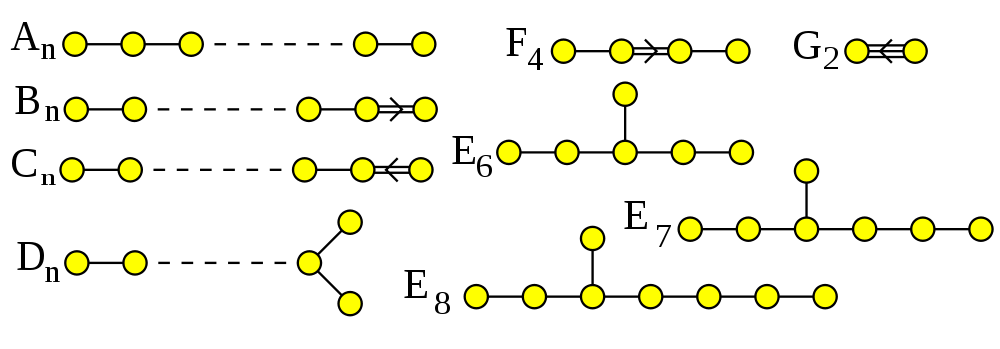
\includegraphics[width=0.7\textwidth]{img/dynkin.png}
\end{center}

A double-edge pointing from $\alpha$ to $\beta$ indicates that
$\frac{||\alpha||}{||\beta||} = \sqrt{2}$. A triple-edge pointing from
$\alpha$ to $\beta$ indicates that $\frac{||\alpha||}{||\beta||} = \sqrt{3}$
(i.e. the arrow points from the larger root to the smaller root).
A single edge indicates that $||\alpha|| = ||\beta||$.

\newpage

We also have,
\begin{itemize}
\item $D_n$,
\[
    \Lambda = \sum_{i=1}^{n-1} \Z (\varepsilon_i - \varepsilon_{i-1})
    + \Z(\varepsilon_{n-1} + \varepsilon_{n}).
\]
\item $F_4$,
\[
    \Lambda = \Z (\varepsilon_2 - \varepsilon_3)
    + \Z(\varepsilon_3 - \varepsilon_4)
    + \Z\varepsilon_4
    + \frac{1}{2} \Z (\varepsilon_1 + \varepsilon_2 + \varepsilon_3 + \varepsilon_4).
\]
\item $G_2 = I_2(6)$,
\[
    \Lambda = \Z (\varepsilon_1 - \varepsilon_2)
    + \Z (-2 \varepsilon_1 + \varepsilon_2 + \varepsilon_3).
\]
\end{itemize}
